\documentclass[conference]{IEEEtran}
\usepackage[utf8]{inputenc}
\usepackage[T5,T1]{fontenc}
\usepackage{cite}
\usepackage{amsmath,amssymb,amsfonts}
\usepackage{graphicx}
\usepackage{booktabs}
\usepackage{array}
\usepackage{multirow}
\usepackage{xcolor}
\usepackage{url}

\newcommand{\vn}[1]{{\fontencoding{T5}\selectfont #1}}

\begin{document}

\title{Automated Visual Quality Inspection with Few Defect Samples: Paradigm Comparison, Protocol Audits, and Few-Shot Reference Diversity on MVTec AD}

\author{
\IEEEauthorblockN{
\vn{Nguyễn Vinh Khánh} (11230549),
\vn{Đỗ Hữu Kiên} (11230552),
\vn{Nguyễn Tống Nguyễn Vũ} (11230604),\\
\vn{Đặng Nhật Huy} (11230544),
\vn{Nguyễn Việt Hoàng} (11230539),
\vn{Nguyễn Tuấn Phong} (11230580)
}
\IEEEauthorblockA{Advisor: \vn{Nguyễn Mạnh Toàn}}
}

\maketitle

\begin{abstract}
Automated visual quality inspection in industrial manufacturing faces severe label scarcity: defect-free parts are abundant, whereas anomalous samples are rare, diverse, and unpredictable. Under a strictly leak-free evaluation protocol across five representative MVTec AD categories (\textit{bottle}, \textit{carpet}, \textit{leather}, \textit{screw}, and \textit{transistor}), this study conducts a controlled comparison of three unsupervised anomaly detection paradigms trained solely on normal images: a Convolutional Autoencoder (\texttt{autoencoder}), a multi-scale PCA plus One-Class SVM (\texttt{one\_class}), and a PatchCore feature-memory model (\texttt{patchcore} and \texttt{patchcore\_refined}). Beyond standard accuracy benchmarking, we audit three critical experimental factors: defect mask truncation under $256\rightarrow 224$ center-cropping, validation-quantile threshold stability under small normal validation sets, and the role of normal-reference diversity versus raw patch count in few-shot learning. Experimental results show that \texttt{patchcore} achieves the highest mean performance ($0.9702$ Image AUROC, $0.9820$ Pixel AUROC, and $0.9291$ Pixel PRO), outperforming \texttt{one\_class} ($0.8046$ Image AUROC) and \texttt{autoencoder} ($0.6823$ Image AUROC, $0.6133$ Pixel PRO). Ground-truth mask auditing confirms zero completely erased defects, though $10.67\%$ of defect masks experience partial border truncation. Bootstrap resampling ($B=1{,}000$) reveals substantial \texttt{P95} recall variance on \textit{screw} ($\sigma = 20.19\%$), while shifting to \texttt{P90} raises mean recall from $82.96\%$ to $94.73\%$ alongside a false-positive rate increase from $10.57\%$ to $18.24\%$. Finally, few-shot subsampling down to $N=10$ normal images shows near-zero degradation on stationary categories (\textit{bottle}: $-0.0016$; \textit{leather}: $-0.0020$) but a $-0.3691$ AUROC collapse on rotated \textit{screw}, demonstrating that normal-reference diversity and memory-bank coverage---rather than raw patch count---govern few-shot generalization.
\end{abstract}

\begin{IEEEkeywords}
Visual anomaly detection, defect localization, MVTec AD, PatchCore, One-Class SVM, Autoencoder, few-shot inspection.
\end{IEEEkeywords}

\section{Introduction}
Visual quality inspection is a foundational requirement in automated manufacturing lines, where surface defects, structural misalignments, and material contamination must be flagged before products reach customers. In real production environments, however, deploying conventional supervised classification or object detection pipelines is hindered by three structural problems. First, factories generate thousands of defect-free (\textit{normal}) items daily, whereas defective samples are scarce, costly to collect, and labor-intensive to annotate with pixel-accurate masks~\cite{bergmann2019mvtec,bergmann2021mvtec}. Second, industrial defects are open-set: anomalies span microscopic scratches on machined threads, subtle weave irregularities on textiles, and missing or bent electronic leads, making closed-set defect taxonomies brittle when novel failure modes emerge~\cite{zou2022spot}. Third, practical inspection systems require not only an image-level pass/fail score, but also spatial defect localization and a decision threshold calibrated strictly on normal validation data without leaking test-set anomalies~\cite{roth2022towards}.

Consequently, visual quality inspection is naturally formulated as \textit{unsupervised} (or \textit{one-class}) anomaly detection and localization, wherein models learn solely from normal training samples and flag deviations at test time. Over the past decade, three distinct algorithmic families have emerged for this task: (i) reconstruction-based networks such as Convolutional Autoencoders~\cite{bergmann2019ssim}, (ii) classical or deep one-class boundary models such as One-Class SVM~\cite{scholkopf2001estimating,ruff2018deep}, and (iii) frozen pretrained feature-memory frameworks exemplified by PatchCore~\cite{roth2022towards}. Yet fair cross-paradigm comparisons are often obscured by inconsistent preprocessing, post-hoc threshold tuning on test data, or aggregate mean scores that hide category-specific failure modes.

In this work, we conduct a controlled empirical comparison of all three paradigms on five MVTec AD categories (\textit{bottle}, \textit{carpet}, \textit{leather}, \textit{screw}, and \textit{transistor}) chosen to span rigid objects, stochastic textures, arbitrarily rotated parts, and multi-component electronics. Every method shares an identical deterministic data split, preprocessing transform, validation-only threshold rule, and standardized evaluation harness covering both image-level detection and pixel-level Per-Region Overlap (PRO)~\cite{bergmann2021mvtec}. In addition, we perform three targeted methodological audits addressing preprocessing validity, quantile threshold stability, and few-shot sample efficiency.

Our main contributions are summarized as follows:
\begin{itemize}
    \item \textbf{Unified Cross-Paradigm Benchmark:} We implement and fairly compare \texttt{autoencoder}, \texttt{one\_class}, and \texttt{patchcore} (plus a higher-capacity \texttt{patchcore\_refined} variant) under a strict zero-test-leakage protocol across image-level, pixel-level, and deployment-cost metrics.
    \item \textbf{Preprocessing Center-Crop Audit:} We quantify the exact geometric impact of standard $256 \rightarrow 224$ center-cropping across all $403$ ground-truth defect masks, identifying when border truncation affects localization and recall.
    \item \textbf{Threshold Stability and Cost Trade-Off Analysis:} Using $1{,}000$-sample validation bootstrapping, we quantify the variance of \texttt{P95} thresholds on small normal validation splits ($42$--$64$ images) and explicitly report both Recall and False-Positive Rate (FPR) across \texttt{P90} versus \texttt{P95} operating points.
    \item \textbf{Few-Shot Diversity Mechanism Analysis:} By combining few-shot subsampling curves ($N \in \{10, 25, 50, 100, \text{full}\}$) with memory-bank dispersion and nearest-neighbor coverage metrics, we show why normal-reference diversity governs few-shot performance more strongly than raw patch count.
\end{itemize}

\section{Related Works}
Research in unsupervised industrial anomaly detection has accelerated substantially since the introduction of the MVTec AD benchmark~\cite{bergmann2019mvtec,bergmann2021mvtec} and subsequent multi-instance datasets such as VisA~\cite{zou2022spot}. Existing methods fall broadly into three methodological paradigms, supplemented by recent normalizing-flow, distillation, and vision-language extensions.

\textbf{Reconstruction-Based Approaches.} Early deep inspection models train autoencoders or generative adversarial networks (GANs) exclusively on normal images so that anomalous regions induce elevated reconstruction error at inference time. Bergmann et al.~\cite{bergmann2019ssim} improved pixel-wise $\ell_2$ autoencoders using structural similarity (SSIM) loss to better preserve local texture geometry. Adversarial variants such as GANomaly~\cite{akcay2018ganomaly} and f-AnoGAN~\cite{schlegl2019fanogan} incorporate latent-space consistency and discriminator features to sharpen reconstructions. More recently, DRAEM~\cite{zavrtanik2021draem} paired a reconstructive sub-network with a discriminative segmentation head trained on synthetic Perlin-noise anomalies. Despite their architectural simplicity and compact storage, pure reconstruction autoencoders frequently suffer from a capacity dilemma: under-parameterized bottlenecks blur stochastic textures (causing false alarms), whereas over-parameterized networks reconstruct subtle defects too faithfully~\cite{bergmann2019mvtec}.

\textbf{One-Class Boundary Methods.} A second lineage frames anomaly detection as estimating the support of the normal distribution. Classical One-Class SVM (OC-SVM)~\cite{scholkopf2001estimating} and Support Vector Data Description (SVDD)~\cite{tax2004support} learn a separating hyperplane or minimum-volume hypersphere around normal feature vectors. Deep SVDD~\cite{ruff2018deep} replaced fixed kernels with an end-to-end neural mapping toward a predefined hypersphere center, while PANDA~\cite{reiss2021panda} showed that adapting ImageNet-pretrained backbones with elastic weight consolidation mitigates feature collapse. Although global pooled CNN representations paired with OC-SVM fit rapidly and require minimal supervision, global pooling discards spatial coordinates, preventing pixel-level localization and attenuating small localized defects.

\textbf{Pretrained Feature-Memory and Embedding Methods.} To avoid catastrophic representation collapse and preserve fine spatial resolution, recent state-of-the-art pipelines leverage frozen ImageNet-pretrained encoders to construct local patch representations. SPADE~\cite{cohen2020sub} aligns multi-resolution CNN feature pyramids and performs pixel-level $k$-nearest-neighbor ($k$-NN) matching against a full training feature gallery, incurring heavy inference cost. PaDiM~\cite{defard2021padim} models each spatial patch location as a multivariate Gaussian distribution, reducing memory overhead via random feature dimensionality selection. PatchCore~\cite{roth2022towards} unifies locally aware mid-level patch aggregation with greedy $k$-center coreset subsampling~\cite{sener2018active} and density-reweighted nearest-neighbor scoring, achieving near-ceiling AUROC and localization with tractable latency. Complementary embedding-based paradigms include conditional normalizing flows such as CFLOW-AD~\cite{gudovskiy2022cflow}, asymmetric student-teacher reverse distillation~\cite{deng2022anomaly}, and CLIP-based zero-/few-shot prompting such as WinCLIP~\cite{jeong2023winclip}.

\textbf{Research Gap.} While prior benchmarks establish that PatchCore outperforms classical reconstruction and global one-class baselines in aggregate AUROC~\cite{roth2022towards}, three practical questions remain under-examined in unified comparative studies: (1) how standard center-crop preprocessing affects ground-truth defect preservation across heterogeneous defect geometries; (2) how reliably quantile thresholds (\texttt{P95} vs.\ \texttt{P90}) generalize when the normal validation pool is small; and (3) whether PatchCore's strong few-shot performance stems from sheer patch multiplicity per image or from the underlying pose and appearance diversity captured in the coreset memory bank. Our study directly investigates these gaps.

\section{Methodology}

\subsection{Research Questions and Hypotheses}
To structure our empirical evaluation beyond raw leaderboard comparisons, we formulate three research questions (\textbf{RQ1}--\textbf{RQ3}) and corresponding hypotheses (\textbf{H1}--\textbf{H3}):
\begin{itemize}
    \item \textbf{RQ1 (Paradigm Trade-offs):} How do reconstruction-based (\texttt{autoencoder}), global one-class (\texttt{one\_class}), and local patch-memory (\texttt{patchcore}) methods compare across object, texture, rotated, and structural defect categories in both accuracy and resource cost?
    \begin{itemize}
        \item \textit{H1:} \texttt{patchcore} will substantially outperform both baselines in detection and pixel localization because mid-level local patch matching avoids texture blurring (which degrades \texttt{autoencoder}) and global spatial averaging (which blinds \texttt{one\_class} to small rotated defects).
    \end{itemize}
    \item \textbf{RQ2 (Preprocessing \& Threshold Validity):} Does standard $256 \rightarrow 224$ center-cropping discard critical defect information, and how stable is validation-only \texttt{P95} thresholding relative to \texttt{P90} under small validation sets?
    \begin{itemize}
        \item \textit{H2:} Center-cropping will preserve image-level labels but partially truncate defects located near image boundaries; meanwhile, \texttt{P95} thresholds derived from $\sim 50$ validation images will exhibit high bootstrap variance on heavy-tailed categories, whereas \texttt{P90} will improve recall at a measurable FPR cost.
    \end{itemize}
    \item \textbf{RQ3 (Few-Shot Reference Diversity):} As normal training samples decrease toward $N=10$, does patch multiplicity alone sustain PatchCore performance, or does degradation depend on category-level pose/appearance diversity and memory-bank coverage?
    \begin{itemize}
        \item \textit{H3:} Because patches within an image are spatially correlated rather than independent observations, categories with low geometric variation will remain robust at $N=10$, whereas categories with wide pose variation (\textit{screw}) will degrade sharply due to incomplete manifold coverage.
    \end{itemize}
\end{itemize}

\subsection{Dataset, Zero-Leakage Protocol, and Preprocessing Audit}
We evaluate on five MVTec AD categories~\cite{bergmann2019mvtec} totaling $1{,}267$ normal training/validation images and $584$ test images ($181$ normal, $403$ defective): \textit{bottle} ($167$ train / $42$ val / $20$ good + $63$ defect test), \textit{carpet} ($224$ / $56$ / $28$ + $89$), \textit{leather} ($196$ / $49$ / $32$ + $92$), \textit{screw} ($256$ / $64$ / $41$ + $119$), and \textit{transistor} ($170$ / $43$ / $60$ + $40$). For every category, \texttt{train/good} is deterministically partitioned into $80\%$ training and $20\%$ normal-only validation (\texttt{seed=42}). The official test set is strictly held out for final reporting; hyperparameters, best checkpoints, and binary decision thresholds are never tuned on test labels.

All images undergo shared preprocessing: bilinear resizing to $256\times 256$, center-cropping to $224\times 224$, and ImageNet normalization. Ground-truth binary masks use nearest-neighbor resizing to $256\times 256$ followed by $224\times 224$ center-cropping. To verify RQ2, we audit all $403$ raw ground-truth defect masks by measuring pixel counts before ($256\times 256$) and after ($224\times 224$) center-cropping, recording the fraction of border-affected images, completely erased masks, and percentage area lost.

\subsection{Compared Anomaly Detection Architectures}
All models inherit a common \texttt{BaseAnomalyMethod} interface consuming identical tensors and exporting image scores (higher means more anomalous) plus optional $[224, 224]$ pixel anomaly maps:
\begin{enumerate}
    \item \textbf{Convolutional Autoencoder (\texttt{autoencoder}):} A four-stage symmetric CNN maps $[3, 224, 224]$ inputs to a $[128, 14, 14]$ latent bottleneck ($\text{base\_channels}=32$). The decoder employs bilinear upsampling followed by $3\times 3$ convolutions (avoiding transposed-convolution checkerboard artifacts). Each per-category model is trained for $40$ epochs (Adam, $\text{lr}=10^{-3}$, weight decay $10^{-5}$, batch size $16$) using combined reconstruction loss $\mathcal{L} = \text{MSE} + 0.5\cdot L_1$, selecting the lowest validation-loss checkpoint. Pixel error maps are smoothed with a Gaussian kernel ($\sigma=2.0$), and image scores equal the mean of the top $2\%$ highest-error pixels (\texttt{topk\_mean}).
    \item \textbf{Multi-Scale One-Class SVM (\texttt{one\_class}):} Using a frozen ImageNet-pretrained \texttt{WideResNet50-2} backbone, we extract feature maps from \texttt{layer2}, \texttt{layer3}, and \texttt{layer4}, apply both Global Average and Global Max Pooling per layer, concatenate, and $\ell_2$-normalize into a $7{,}168$-dimensional descriptor. Features are standardized (\texttt{StandardScaler}), compressed via \texttt{PCA} retaining $95\%$ variance ($137$--$206$ dimensions across categories), and fit with an RBF \texttt{OneClassSVM} ($\nu=0.05$, $\gamma=\text{'scale'}$). Because the validation set contains no defects, $\nu=0.05$ aligns directly with the $5\%$ tail of the \texttt{P95} threshold rule. Image scores are computed as $s(x) = -f_{\text{decision}}(x)$.
    \item \textbf{PatchCore Memory Bank (\texttt{patchcore} \& \texttt{patchcore\_refined}):} Following Roth et al.~\cite{roth2022towards}, intermediate \texttt{WideResNet50-2} maps (\texttt{layer2} and \texttt{layer3}) are smoothed via $3\times 3$ average pooling ($\text{stride}=1$), bilinearly aligned to a $28\times 28$ grid ($1{,}536$ channels), and projected via a deterministic random orthogonalized matrix to $D=384$. Across $167$--$256$ training images, this yields $130{,}928$--$200{,}704$ raw patches per category. We apply $k$-Center Greedy coreset subsampling~\cite{sener2018active} configured at ratio $0.10$ with cap $M_{\max}=10{,}000$ patches/category (yielding effective retention ratios of $4.98\%$--$7.64\%$). Test patches are scored by nearest-neighbor Euclidean distance to the coreset, reweighted using $k=9$ local density neighbors (PatchCore Eq.~6), and upsampled to $224\times 224$ with Gaussian smoothing ($\sigma=4.0$). We also evaluate a higher-capacity variant, \texttt{patchcore\_refined}, increasing projection dimension to $D=512$, coreset cap to $M_{\max}=15{,}000$ ($7.47\%$--$11.46\%$ retention), $k=5$, and $\sigma=3.5$.
\end{enumerate}

\subsection{Evaluation, Bootstrap Stability, and Diversity Metrics}
Image-level discrimination is measured via threshold-free \textbf{Image AUROC}, alongside \textbf{Precision}, \textbf{Recall}, \textbf{F1}, and \textbf{FPR} evaluated at the category-specific validation $95$th percentile $\tau_c = \text{Percentile}_{95}(\{s_i \mid i \in \text{val}_c\})$. Pixel-level localization is evaluated via \textbf{Pixel AUROC} and \textbf{Per-Region Overlap (PRO)}~\cite{bergmann2021mvtec}, which weights each connected ground-truth defect component equally and integrates the mean region overlap curve over $\text{FPR} \in [0, 0.3]$ normalized by $0.3$.

To assess threshold stability (RQ2), we perform $B=1{,}000$ bootstrap resamples of each category's validation normal scores ($n_{\text{val}} \in [42, 64]$), recomputing $\tau_b$ at both \texttt{P90} and \texttt{P95} and reporting standard deviations and $95\%$ confidence intervals (CIs) for threshold, Recall, and FPR. For few-shot analysis (RQ3), training sets are deterministically subsampled to $N \in \{10, 25, 50, 100, \text{full}\}$ images per category (\texttt{seed=42}) while keeping validation and test splits unchanged. To characterize normal-manifold spread across categories, we compute three geometric statistics on each category's saved full PatchCore coreset memory bank: mean $\ell_2$ dispersion from the bank centroid, spectral effective rank $\exp(-\sum_i p_i \log p_i)$ of centered singular values, and mean $5$-NN intra-bank coverage radius.

\section{Results}

\subsection{Overall Cross-Paradigm Comparison}
Table~\ref{tab:main_comparison} summarizes mean performance and computational footprint across the five MVTec AD categories. \texttt{patchcore} dominates image-level detection ($0.9702$ Image AUROC, $0.8692$ F1) and pixel-level localization ($0.9820$ Pixel AUROC, $0.9291$ Pixel PRO), surpassing \texttt{autoencoder} by $+0.2879$ Image AUROC and $+0.3158$ Pixel PRO. \texttt{one\_class} ranks second in detection ($0.8046$ Image AUROC, $0.7149$ F1) with the fastest fitting time ($51.30\,\text{s}$ total), though it provides no pixel maps. \texttt{autoencoder} achieves the lowest inference latency ($47.41\,\text{ms/img}$) and smallest checkpoint ($3.40\,\text{MB/cat}$), but incurs the longest training time ($2{,}410.60\,\text{s}$) and highest false-positive rate ($0.3295$). Meanwhile, \texttt{patchcore\_refined} reduces mean FPR to $0.0896$ and marginally lifts Pixel PRO ($0.9298$) at roughly double the artifact size ($29.92\,\text{MB/cat}$).

\begin{table*}[t]
\centering
\caption{Mean Benchmark Performance and Resource Footprint Across Five MVTec AD Categories (Val \texttt{P95} Threshold)}
\label{tab:main_comparison}
\footnotesize
\setlength{\tabcolsep}{4.0pt}
\resizebox{\textwidth}{!}{%
\begin{tabular}{@{}lcccccccccc@{}}
\toprule
\textbf{Method / Run} & \textbf{Img AUROC}$\uparrow$ & \textbf{F1}$\uparrow$ & \textbf{Prec.}$\uparrow$ & \textbf{Recall}$\uparrow$ & \textbf{FPR}$\downarrow$ & \textbf{Pix AUROC}$\uparrow$ & \textbf{Pix PRO}$\uparrow$ & \textbf{ms/img}$\downarrow$ & \textbf{MB/cat}$\downarrow$ & \textbf{Fit (s)}$\downarrow$ \\
\midrule
\texttt{autoencoder}       & 0.6823 & 0.5212 & 0.8097 & 0.4734 & 0.3295 & 0.7916 & 0.6133 & \textbf{47.41} & \textbf{3.40} & 2410.60 \\
\texttt{one\_class}         & 0.8046 & 0.7149 & 0.8022 & 0.7007 & 0.1972 & ---    & ---    & 52.74          & 9.48          & \textbf{51.30} \\
\texttt{patchcore}         & \textbf{0.9702} & \textbf{0.8692} & 0.9441 & \textbf{0.8296} & 0.1057 & \textbf{0.9820} & 0.9291 & 56.99 & 15.66 & 310.53 \\
\texttt{patchcore\_refined}& 0.9674 & 0.8519 & \textbf{0.9462} & 0.7974 & \textbf{0.0896} & 0.9819 & \textbf{0.9298} & 59.89 & 29.92 & 566.11 \\
\bottomrule
\end{tabular}%
}
\end{table*}

\subsection{Per-Category Breakdown and Pixel Localization}
Category-level metrics in Table~\ref{tab:per_category} reveal stark mechanistic contrasts behind the aggregate means. On stationary surfaces, \texttt{one\_class} performs strongly (\textit{leather}: $1.0000$, \textit{bottle}: $0.9623$, \textit{carpet}: $0.9516$), yet collapses to $0.4036$ Image AUROC on \textit{screw} because global average/max pooling blurs tiny head and thread scratches across $360^\circ$ rotations. Conversely, \texttt{autoencoder} localizes smooth \textit{leather} reasonably well ($0.9634$ Pixel AUROC, $0.8997$ PRO) but fails on stochastic textile weave (\textit{carpet}: $0.4438$ Image AUROC, $0.3196$ PRO), where high-frequency normal threads inflate reconstruction residuals. \texttt{patchcore} maintains $>0.93$ Image AUROC and $>0.90$ PRO across all five categories, reaching $1.0000$ Image AUROC on \textit{bottle} and $0.9638$ on \textit{transistor}. Increasing memory capacity in \texttt{patchcore\_refined} specifically boosts \textit{screw} F1 from $0.6667$ to $0.7128$ and \textit{screw} PRO from $0.9156$ to $0.9227$, though at lower recall on \textit{transistor} ($0.5250$ vs.\ $0.7000$) under \texttt{P95}. Qualitative inspection of \textit{screw} heatmaps (Fig.~\ref{fig:gallery_screw}) confirms that \texttt{patchcore} sharply isolates fine scratches and manipulated fronts whereas \texttt{autoencoder} exhibits elevated background residuals along screw threads.

\begin{table}[t]
\centering
\caption{Per-Category Image AUROC and Pixel Localization (AUROC / PRO)}
\label{tab:per_category}
\footnotesize
\setlength{\tabcolsep}{3.0pt}
\resizebox{\columnwidth}{!}{%
\begin{tabular}{@{}lcccc@{}}
\toprule
\textbf{Category} & \textbf{AE} & \textbf{OC-SVM} & \textbf{PatchCore} & \textbf{PC-Refined} \\
\midrule
\multicolumn{5}{@{}l}{\textit{Image-Level AUROC}} \\
\textit{bottle}     & 0.8897 & 0.9623 & \textbf{1.0000} & \textbf{1.0000} \\
\textit{carpet}     & 0.4438 & 0.9516 & 0.9575 & \textbf{0.9595} \\
\textit{leather}    & 0.7687 & \textbf{1.0000} & 0.9976 & 0.9973 \\
\textit{screw}      & 0.7649 & 0.4036 & \textbf{0.9324} & 0.9258 \\
\textit{transistor} & 0.5446 & 0.7054 & \textbf{0.9638} & 0.9546 \\
\midrule
\multicolumn{5}{@{}l}{\textit{Pixel-Level AUROC / Pixel PRO}} \\
\textit{bottle}     & 0.793 / 0.559 & --- & \textbf{0.982 / 0.920} & 0.981 / 0.916 \\
\textit{carpet}     & 0.586 / 0.320 & --- & \textbf{0.983 / 0.909} & 0.983 / 0.909 \\
\textit{leather}    & 0.963 / 0.900 & --- & \textbf{0.990 / 0.965} & 0.989 / 0.964 \\
\textit{screw}      & 0.948 / 0.808 & --- & 0.983 / 0.916 & \textbf{0.984 / 0.923} \\
\textit{transistor} & 0.668 / 0.480 & --- & 0.971 / 0.937 & \textbf{0.972 / 0.937} \\
\bottomrule
\end{tabular}%
}
\end{table}

\begin{figure}[t]
\centering
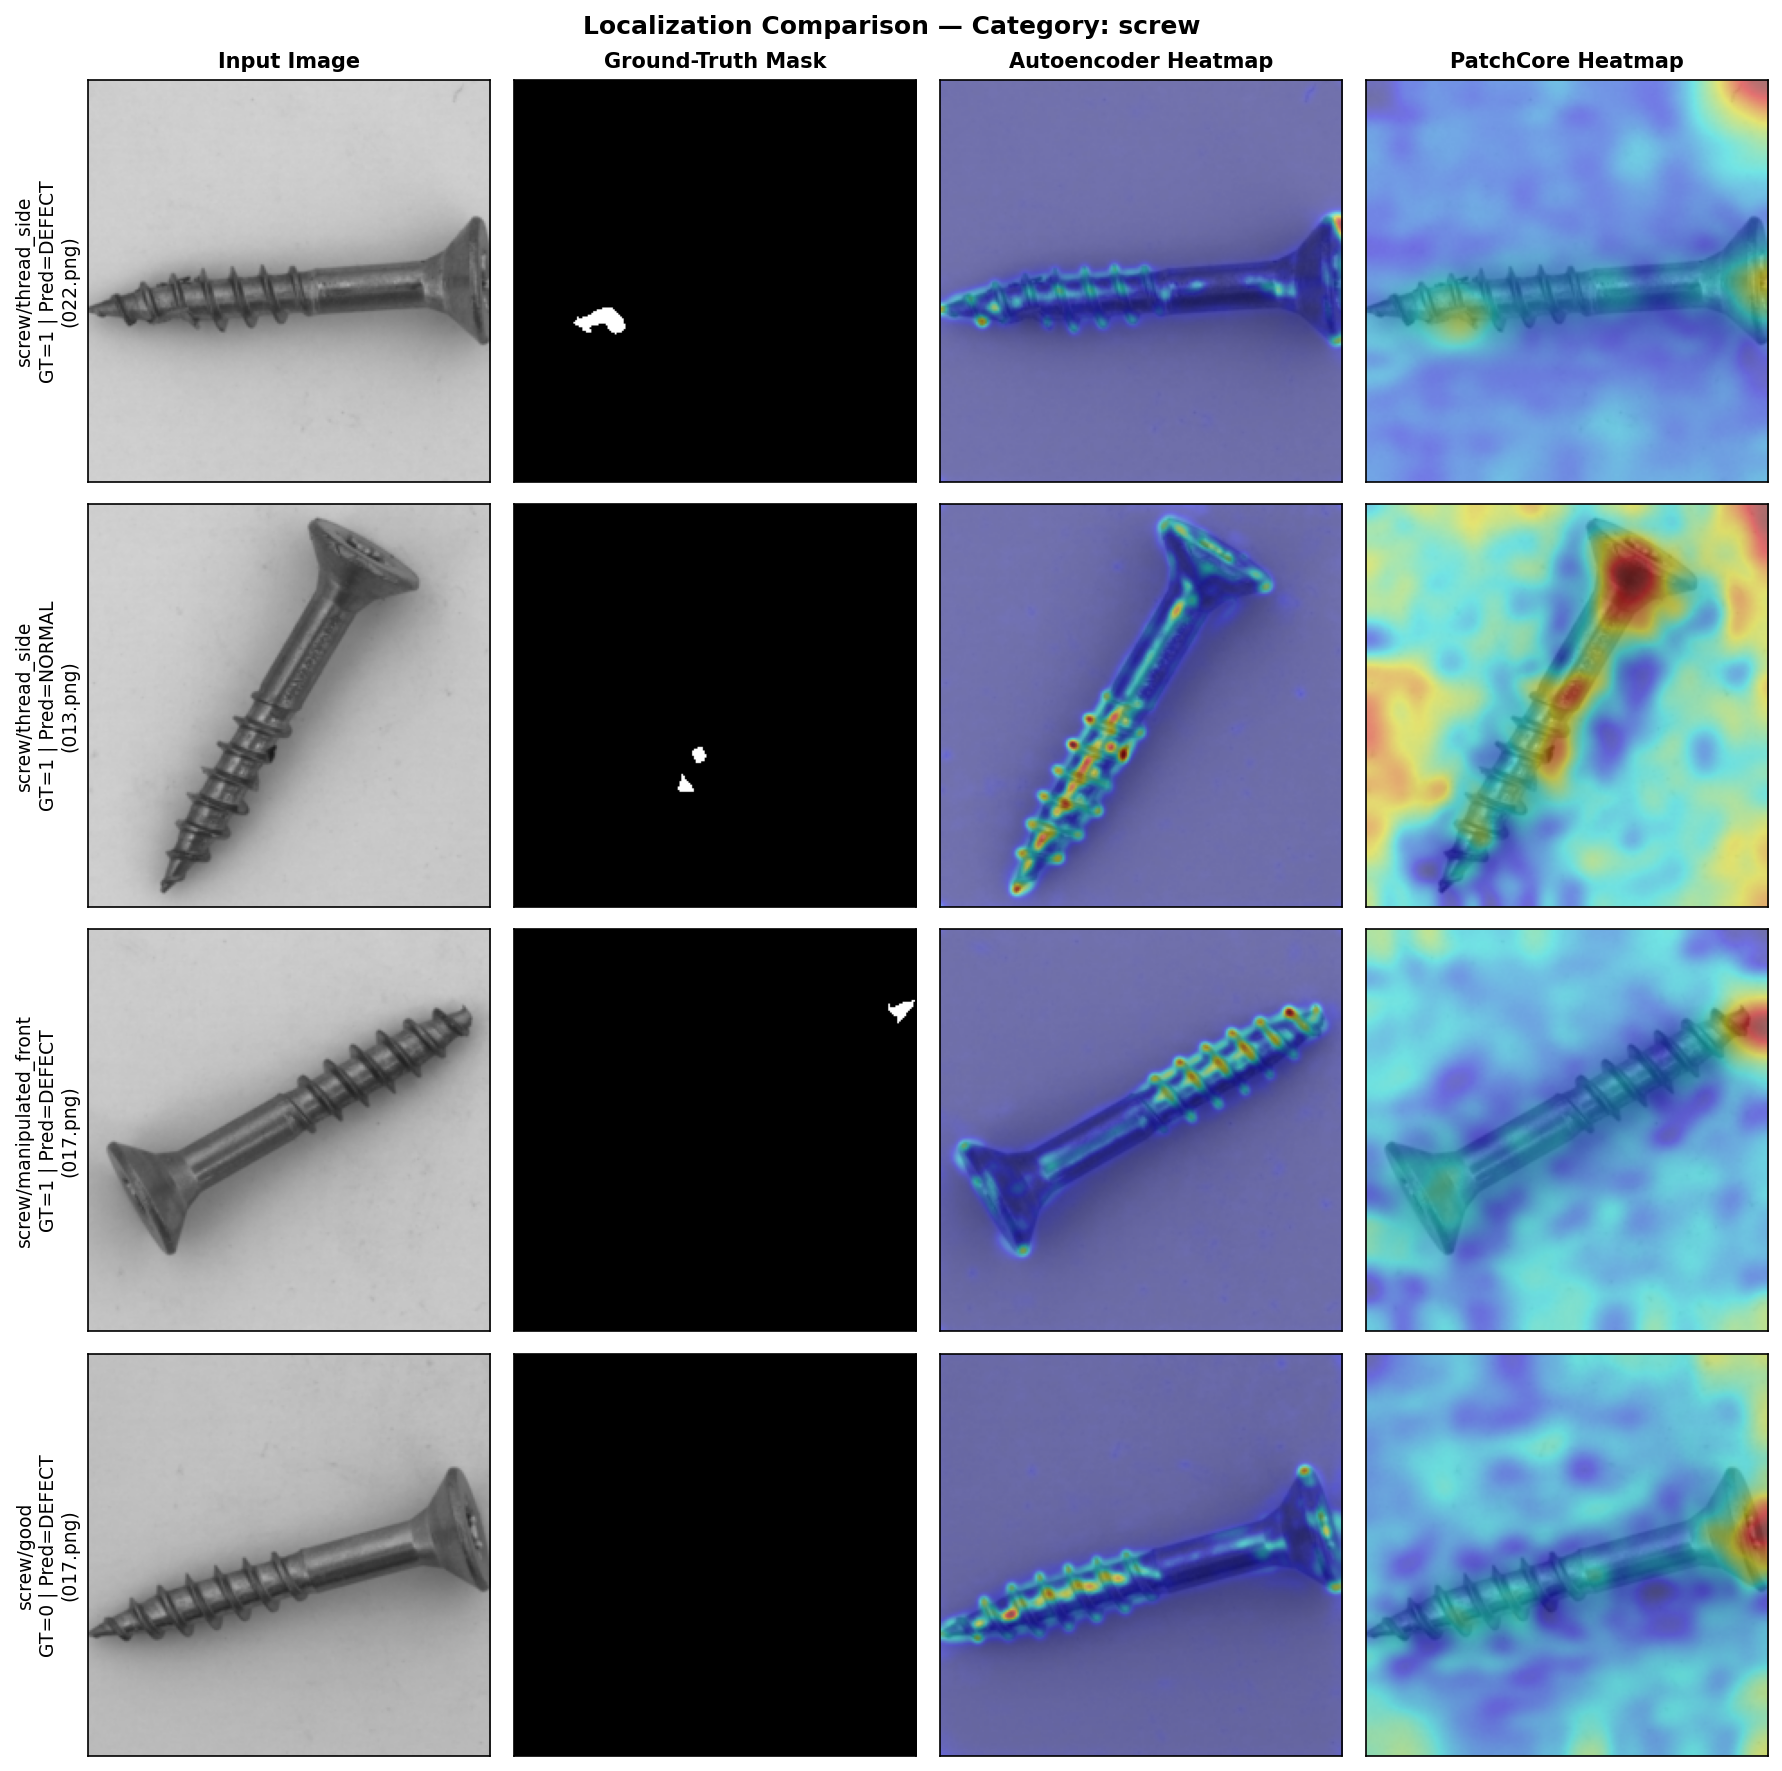
\includegraphics[width=\linewidth]{figures/gallery_screw.png}
\caption{Qualitative defect localization on \textit{screw} (Input, Ground Truth, Autoencoder error map, and PatchCore anomaly map). PatchCore pinpoints localized tip and thread defects with minimal background noise.}
\label{fig:gallery_screw}
\end{figure}

\subsection{Preprocessing Center-Crop Audit}
Auditing all $403$ ground-truth defect masks under \texttt{Resize(256)+CenterCrop(224)} (Fig.~\ref{fig:crop_audit}) shows that \textbf{zero} defect masks are completely erased ($0/403$), preserving image-level defect ground truth across the benchmark. However, $43$ of $403$ defect images ($10.67\%$) touch the cropped border and lose part of their anomalous region, with an overall mean mask area loss of $1.69\%$ (and $15.79\%$ among the $43$ affected images). Border truncation concentrates heavily in specific failure modes: $22.50\%$ ($9/40$) of \textit{transistor} defect images (specifically $60.0\%$ of \textit{misplaced} and $30.0\%$ of \textit{bent\_lead}, losing up to $38.12\%$ mask area), $12.36\%$ ($11/89$) of \textit{carpet} images (up to $65.22\%$ on \textit{color}), and $9.24\%$ ($11/119$) of \textit{screw} images---all $11$ occurring in \textit{manipulated\_front} ($45.83\%$ of that defect type, losing up to $53.70\%$ area). \textit{Leather} ($8.70\%$) and \textit{bottle} ($6.35\%$) exhibit smaller border effects.

\begin{figure}[t]
\centering
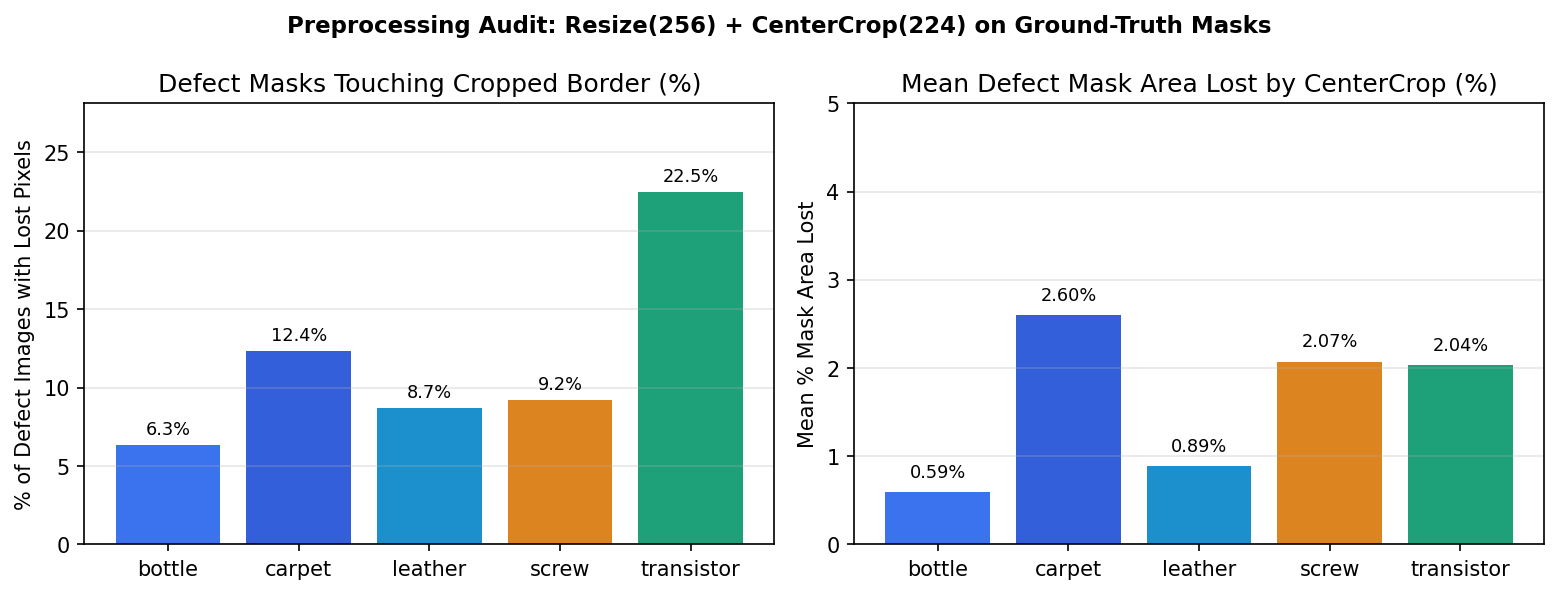
\includegraphics[width=\linewidth]{figures/preprocessing_crop_audit.png}
\caption{Ground-truth mask audit for $256 \rightarrow 224$ center-cropping across $403$ defect images: percentage of border-affected images (left) and mean mask area lost (right).}
\label{fig:crop_audit}
\end{figure}

\subsection{Threshold Stability and P90 vs.\ P95 Operating Points}
Table~\ref{tab:p90_p95} and Fig.~\ref{fig:threshold_stability} quantify both validation-quantile bootstrap uncertainty ($B=1{,}000$) and the explicit Recall--FPR trade-off between \texttt{P90} and \texttt{P95}. Because validation sets contain only $42$--$64$ normal images, \texttt{P95} estimates rely on the upper $2$--$3$ normal samples, producing wide $95\%$ bootstrap confidence intervals on heavy-tailed categories. Specifically, for \texttt{patchcore} at \texttt{P95}, \textit{screw} ($n_{\text{val}}=64$) yields $50.42\%$ Recall with $\sigma = 20.19\%$ ($95\%$ CI: $[16.81\%, 80.67\%]$), and \textit{transistor} ($n_{\text{val}}=43$) yields $70.00\%$ Recall with $\sigma = 20.10\%$ ($95\%$ CI: $[40.00\%, 100.00\%]$).

Shifting the operating point from \texttt{P95} to \texttt{P90} consistently increases Recall across all methods, but always carries an explicit FPR penalty: on \texttt{patchcore}, mean Recall rises by $+11.77\%$ ($82.96\% \rightarrow 94.73\%$, driven by \textit{screw} $50.42\% \rightarrow 78.15\%$ and \textit{transistor} $70.00\% \rightarrow 100.00\%$), while mean FPR rises by $+7.67\%$ ($10.57\% \rightarrow 18.24\%$, notably \textit{carpet} $25.00\% \rightarrow 39.29\%$ and \textit{leather} $18.75\% \rightarrow 31.25\%$). Across the baselines, \texttt{patchcore\_refined} shows a smaller Recall gain ($79.74\% \rightarrow 84.55\%$) for $+8.00\%$ FPR, \texttt{one\_class} gains $+2.13\%$ Recall for $+9.06\%$ FPR, and \texttt{autoencoder} gains $+3.36\%$ Recall at an already high FPR ($32.95\% \rightarrow 34.26\%$).

\begin{table}[t]
\centering
\caption{P90 vs.\ P95 Operating Point Trade-off (Recall, FPR) and P95 Bootstrap Std}
\label{tab:p90_p95}
\scriptsize
\setlength{\tabcolsep}{2.5pt}
\resizebox{\columnwidth}{!}{%
\begin{tabular}{@{}lccccccc@{}}
\toprule
\textbf{Run / Scope} & \multicolumn{2}{c}{\textbf{P90}} & \multicolumn{2}{c}{\textbf{P95}} & \textbf{$\Delta$Rec} & \textbf{$\Delta$FPR} & \textbf{Rec Std} \\
\cmidrule(lr){2-3} \cmidrule(lr){4-5}
 & \textbf{Rec} & \textbf{FPR} & \textbf{Rec} & \textbf{FPR} & \textbf{(P90-95)} & \textbf{(P90-95)} & \textbf{(P95)} \\
\midrule
\texttt{autoencoder} (mean)        & 0.507 & 0.343 & 0.473 & 0.330 & +0.034 & +0.013 & 0.034 \\
\texttt{one\_class} (mean)         & 0.722 & 0.288 & 0.701 & 0.197 & +0.021 & +0.091 & 0.031 \\
\texttt{patchcore\_ref.} (mean)    & 0.845 & 0.170 & 0.797 & 0.090 & +0.048 & +0.080 & 0.073 \\
\texttt{patchcore} (mean)          & 0.947 & 0.182 & 0.830 & 0.106 & +0.118 & +0.077 & 0.087 \\
\midrule
\textit{PC: bottle} ($n=42$)       & 1.000 & 0.050 & 1.000 & 0.000 &  0.000 & +0.050 & 0.000 \\
\textit{PC: carpet} ($n=56$)       & 0.955 & 0.393 & 0.944 & 0.250 & +0.011 & +0.143 & 0.027 \\
\textit{PC: leather} ($n=49$)      & 1.000 & 0.313 & 1.000 & 0.188 &  0.000 & +0.125 & 0.006 \\
\textit{PC: screw} ($n=64$)        & 0.782 & 0.073 & 0.504 & 0.024 & +0.277 & +0.049 & 0.202 \\
\textit{PC: transistor} ($n=43$)   & 1.000 & 0.083 & 0.700 & 0.067 & +0.300 & +0.017 & 0.201 \\
\bottomrule
\end{tabular}%
}
\end{table}

\begin{figure}[t]
\centering
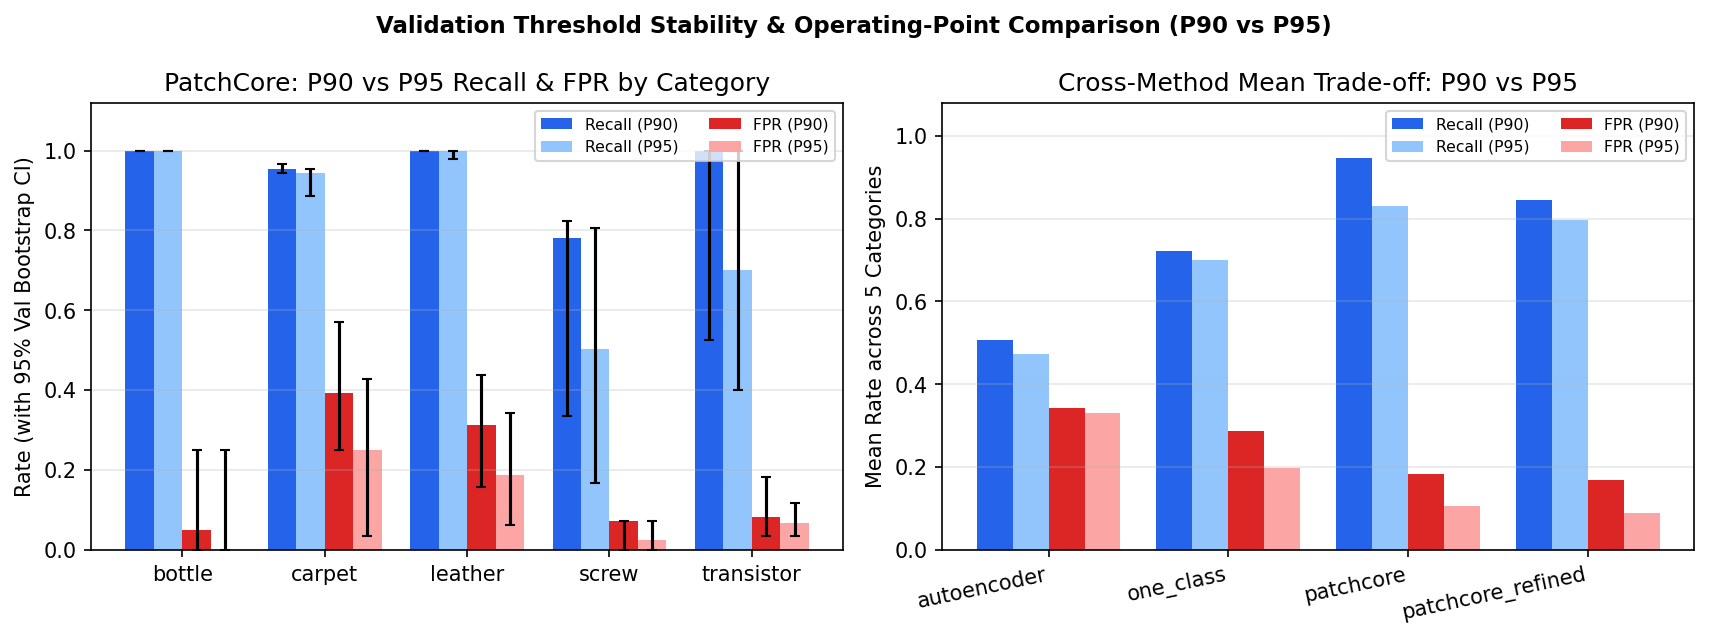
\includegraphics[width=\linewidth]{figures/threshold_stability_p90_p95.png}
\caption{Bootstrap $95\%$ CI stability on PatchCore per category (left) and cross-method mean Recall vs.\ FPR comparison at \texttt{P90} and \texttt{P95} (right).}
\label{fig:threshold_stability}
\end{figure}

\subsection{Few-Shot Sensitivity and Memory-Bank Diversity}
At the aggregate mean level, reducing normal training samples from Full ($167$--$256$ images) down to $N=10$ lowers \texttt{patchcore} Image AUROC from $0.9702$ to $0.8793$ and Pixel PRO from $0.9291$ to $0.8862$---still ahead of full-data \texttt{one\_class} ($0.8046$ Image AUROC) and \texttt{autoencoder} ($0.6823$ Image AUROC, $0.6133$ PRO). However, per-category decomposition (Table~\ref{tab:fewshot} and Fig.~\ref{fig:fewshot_div}) shows that this average masks dramatic divergence despite every category receiving an identical raw budget of $10 \times 28 \times 28 = 7{,}840$ patch embeddings at $N=10$.

Specifically, categories with consistent global alignment or homogeneous texture suffer minimal loss at $N=10$: \textit{bottle} drops by only $0.0016$ ($1.0000 \rightarrow 0.9984$), \textit{leather} by $0.0020$ ($0.9976 \rightarrow 0.9956$), and \textit{carpet} by $0.0221$ ($0.9575 \rightarrow 0.9354$), while their Pixel PRO remains virtually unchanged ($\le 0.001$ drop). In contrast, \textit{transistor} drops by $0.0600$ ($0.9638 \rightarrow 0.9038$) and \textit{screw} suffers a severe $-0.3691$ AUROC collapse ($0.9324 \rightarrow 0.5632$, with PRO dropping $-0.1728$ from $0.9156 \rightarrow 0.7428$). Geometric inspection of the full PatchCore coreset banks explains why: \textit{screw} and \textit{transistor} exhibit substantially higher $\ell_2$ patch dispersion ($10.85$ and $10.31$) and sparser intra-bank $5$-NN coverage radii ($6.97$ and $7.54$) than \textit{leather} ($6.38$ dispersion, $5.53$ radius) or \textit{bottle} ($5.25$ radius). Because \textit{screw} undergoes arbitrary $360^\circ$ orientations across $256$ training images, $10$ normal images span only a sparse subset of rotational modes, leaving unseen normal orientations out-of-distribution relative to the memory bank.

\begin{table}[t]
\centering
\caption{PatchCore Few-Shot Degradation ($N=10$ vs.\ Full) and Full Memory-Bank Geometric Diversity}
\label{tab:fewshot}
\scriptsize
\setlength{\tabcolsep}{2.5pt}
\resizebox{\columnwidth}{!}{%
\begin{tabular}{@{}lcccccc@{}}
\toprule
\textbf{Category} & \textbf{AUROC} & \textbf{AUROC} & \textbf{Drop} & \textbf{PRO} & \textbf{Bank} & \textbf{5-NN} \\
 & \textbf{(N=10)} & \textbf{(Full)} & \textbf{(Full-10)} & \textbf{(N=10)} & \textbf{Disp.} & \textbf{Radius} \\
\midrule
\textit{bottle}     & 0.9984 & 1.0000 & 0.0016 & 0.9241 & 9.36  & 5.25 \\
\textit{carpet}     & 0.9354 & 0.9575 & 0.0221 & 0.9102 & 6.75  & 5.93 \\
\textit{leather}    & 0.9956 & 0.9976 & 0.0020 & 0.9643 & 6.38  & 5.53 \\
\textit{screw}      & 0.5632 & 0.9324 & \textbf{0.3691} & 0.7428 & \textbf{10.85} & 6.97 \\
\textit{transistor} & 0.9038 & 0.9638 & 0.0600 & 0.8894 & 10.31 & \textbf{7.54} \\
\bottomrule
\end{tabular}%
}
\end{table}

\begin{figure}[t]
\centering
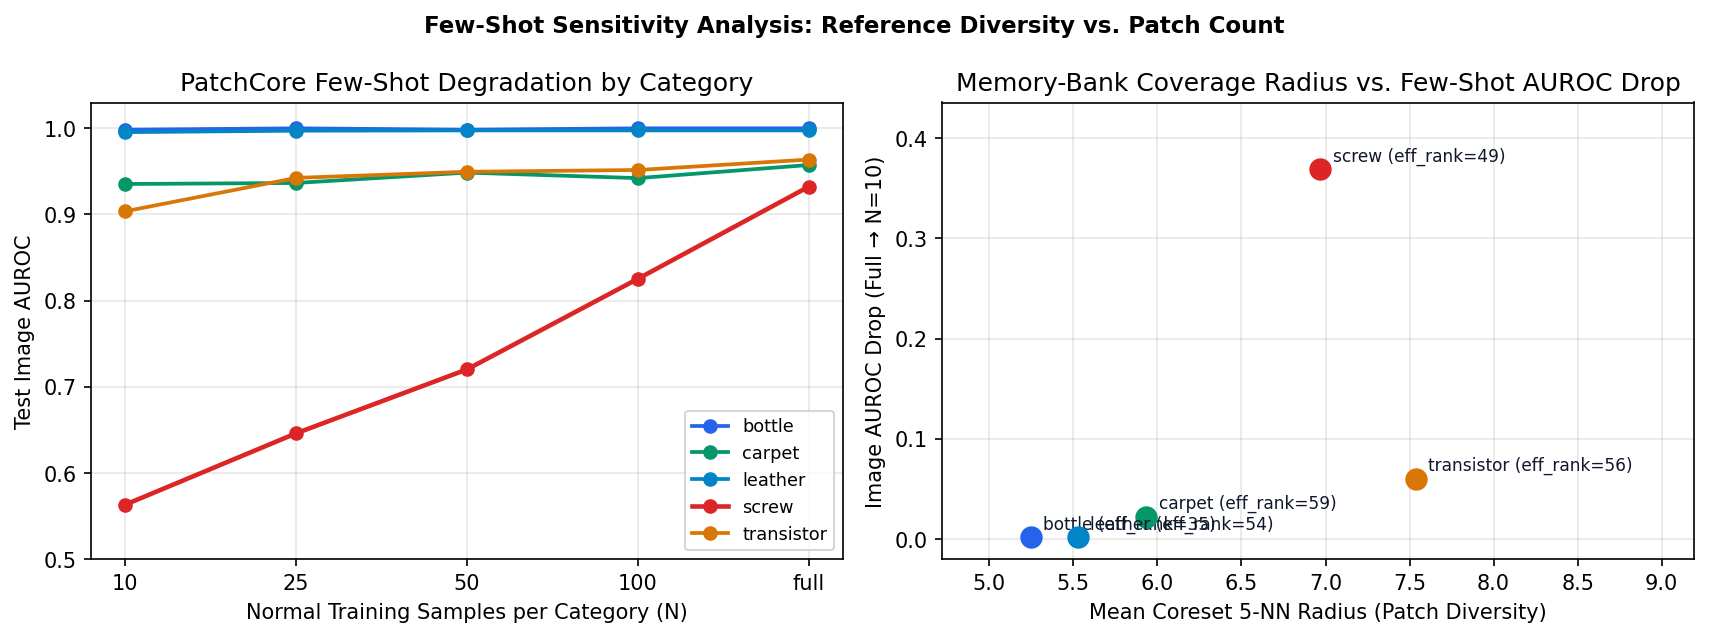
\includegraphics[width=\linewidth]{figures/fewshot_category_degradation.png}
\caption{Per-category PatchCore few-shot Image AUROC curves from $N=10$ to Full (left) and full memory-bank $5$-NN coverage radius versus few-shot AUROC drop (right).}
\label{fig:fewshot_div}
\end{figure}

\section{Discussion}

\subsection{Evaluation of Hypotheses and Mechanistic Findings}
Our empirical findings confirm \textbf{H1}: local mid-level feature memory (\texttt{patchcore}) avoids both the texture-reconstruction noise of \texttt{autoencoder} on \textit{carpet} ($0.9575$ vs.\ $0.4438$) and the spatial-averaging blindness of \texttt{one\_class} on \textit{screw} ($0.9324$ vs.\ $0.4036$). Increasing coreset density in \texttt{patchcore\_refined} improves fine-defect separation on \textit{screw} ($\text{F1}: 0.6667 \rightarrow 0.7128$) and reduces mean FPR ($10.57\% \rightarrow 8.96\%$), though the smaller neighborhood ($k=5$) slightly raises \texttt{P95} sensitivity on \textit{transistor}.

Our audits also support \textbf{H2}. Although $256\rightarrow 224$ center-cropping never eliminates an entire defect label ($0/403$), truncating $22.50\%$ of \textit{transistor} and $45.83\%$ of \textit{screw/manipulated\_front} masks removes informative peripheral pixels---precisely on the categories where recall is hardest to maintain. Similarly, bootstrapping demonstrates that \texttt{P95} thresholds estimated from $42$--$64$ normal validation images exhibit $\sim 20\%$ recall standard deviation on \textit{screw} and \textit{transistor}. Moving to \texttt{P90} recovers $+11.77\%$ mean Recall on \texttt{patchcore} ($+27.73\%$ on \textit{screw}), confirming that operating-point selection must balance miss cost against a $+7.67\%$ FPR increase rather than treating \texttt{P95} as universally optimal.

Finally, our few-shot analysis validates \textbf{H3} and refines the interpretation of patch-based sample efficiency. Having $7{,}840$ patch embeddings from $N=10$ images does not equate to $7{,}840$ independent observations: intra-image patches are spatially correlated, and repeated views of aligned parts (\textit{bottle}, \textit{leather}) yield redundant descriptors. Consequently, few-shot generalization succeeds when the $N$ normal reference images adequately cover the manifold of normal poses and appearances. Where normal variation is high (\textit{screw}), $N=10$ leaves large gaps in coreset coverage and degrades toward near-random image ranking ($0.5632$ AUROC).

\subsection{Limitations}
Several methodological limitations must be noted when interpreting these results:
\begin{enumerate}
    \item \textbf{Single-Seed Few-Shot Subsampling:} Sensitivity experiments across $N \in \{10, 25, 50, 100\}$ were executed with a single deterministic seed (\texttt{seed=42}) per category, leaving run-to-run subset selection variance at $N=10$ unquantified.
    \item \textbf{Center-Crop Border Truncation:} Adhering to the standard $256\rightarrow 224$ center-crop protocol truncated border pixels on $10.67\%$ of defect masks, potentially depressing recall on peripheral defects.
    \item \textbf{Small-Validation Quantile Variance:} With $n_{\text{val}} \in [42, 64]$, empirical tail quantiles (\texttt{P95}) are inherently noisy, as confirmed by our bootstrap intervals.
    \item \textbf{Full-Coreset Diversity Proxy:} Memory-bank geometric dispersion and $5$-NN radius were measured on the saved full-training coreset artifacts rather than per-$N$ subsampled memory banks, providing an indirect structural proxy for category manifold complexity.
    \item \textbf{Lack of Rotation Equivariance:} \texttt{patchcore} relies on canonical CNN patch features without rotation alignment or multi-angle augmentation, making few-shot generalization vulnerable on arbitrarily oriented objects such as \textit{screw}.
\end{enumerate}

\subsection{Future Works}
Building directly on these findings, future work should pursue four concrete improvements: (1) replacing center-cropping with aspect-preserving padding or full-resolution sliding-window patch extraction so peripheral defects on \textit{transistor} and \textit{screw} are never truncated; (2) evaluating multi-seed few-shot sampling alongside diversity-maximizing normal reference selection (e.g., selecting the $N$ most visually diverse normal images via clustering or $k$-center selection at the image level) and controlled rotation augmentation for unaligned parts; (3) replacing raw empirical \texttt{P95} quantiles with extreme-value theory (EVT) tail modeling or conformal calibration to stabilize operating thresholds on small normal validation pools; and (4) extending the comparison to modern normal-only distillation~\cite{deng2022anomaly} and vision-language baselines~\cite{jeong2023winclip} across larger multi-object benchmarks such as VisA~\cite{zou2022spot}.

\bibliographystyle{IEEEtran}
\bibliography{references}

\end{document}
